\documentclass[a4paper, 12pt]{report}
\usepackage{cmap}
\usepackage[T2A]{fontenc}
\usepackage[utf8]{inputenc}
\usepackage[english,russian]{babel}
\usepackage{listings}
\usepackage{amsmath}
\usepackage{float}
\usepackage{csquotes}
\usepackage{graphicx}
\graphicspath{ {./images/} }
\usepackage{xcolor}
\definecolor{buzzlightyear}{HTML}{8757A5}
\definecolor{grass}{HTML}{738D06}
\definecolor{literal}{HTML}{F18A2B}
\definecolor{commentcolor}{HTML}{8E908B}

\lstdefinestyle{habrstyle}{
	backgroundcolor=\color{white},
	commentstyle=\color{commentcolor},
	keywordstyle=\bfseries\color{buzzlightyear},
	numberstyle=\tiny\color{commentcolor},
	stringstyle=\color{grass},
	basicstyle=\ttfamily\footnotesize,
	breakatwhitespace=false,         
    	breaklines=true,                 
   	captionpos=b,                    
    	keepspaces=true,                 
    	numbers=left,                    
    	numbersep=7pt,                  
    	showspaces=false,                
    	showstringspaces=false,
   	showtabs=false,                  
    	tabsize=4
}

\lstset{style=habrstyle}

\author{3530901/80201, Шелаев Н. Р.}
\title{Лабораторная работа № 2. Гармоники.}
\date{\today}

\begin{document}
	\maketitle
	\tableofcontents
	\listoffigures
	\lstlistoflistings

	\chapter{Основные свойства преобразования Фурье}
	\section{Общие формулы}
	Формулы для прямого и обратного преобразования Фурье (ПФ и ОПФ). Сигнал $f(t)$:
	\[
        		\begin{aligned}
            		\text{Прямое: } && \Phi_i(\nu) &= \int_{-\infty}^{\infty} \phi(t) e^{-2\pi i\nu t} dt \\
            		\text{Обратное: } && \phi(t) &=  \int_{-\infty}^{\infty} \Phi_i(\nu) e^{2\pi i\nu t} d\nu
        		\end{aligned}
    	\]
	\section{Свойства}
    	\subsection{Суммирование функций}
	Преобразование Фурье - линейное преобразование. Отсюда следует, что ПФ линейной комбинации некоторых функций равно аналогичной линейной комбинации ПФ этих функций.
	\[
        		\begin{aligned}
            		 \sum_{i = 1}^{n}\alpha_i\phi_i(t) \leftrightarrow \sum_{i = 1}^{n}\alpha_i\Phi_i(\nu)
        		\end{aligned}
    	\]

	\subsection{Смещение функций}
	При смещении функции по аргументу на $\Delta t$ её ПФ умножается на $e^{2\pi i \nu\Delta t}$. Пусть $t' = t + \Delta t$, тогда:
	\[
        		\begin{aligned}
            		\phi(t + \Delta t) \leftrightarrow \int_{-\infty}^{\infty} \phi(t + \Delta t) e^{-2\pi i\nu t} dt
			&= \int_{-\infty}^{\infty} \phi(t') e^{-2\pi i\nu (t' - \Delta t)} dt \\
			&= e^{2\pi i\nu\Delta t} \cdot \Phi_i(\nu)
        		\end{aligned}
    	\]

	\subsection{Изменение масштаба аргумента функции}
	Если аргумент $t$ функции $\phi(t)$ заменить на $\alpha t$, где $\alpha$ - постоянный коэффициент, то ПФ функции с $\Phi_i(\nu)$ изменится на $\frac{1}{|\alpha|} \Phi\left(\frac{\nu}{\alpha}\right)$. Это доказывается заменой $t' = \alpha t$:
	\[
        		\begin{aligned}
            		\phi(\alpha t) \leftrightarrow \int_{-\infty}^{\infty} \phi(\alpha t) e^{-2\pi i\nu t} dt
            		&= \frac{1}{|\alpha|} \dot \int_{-\infty}^{\infty} \phi(t') e^{-2\pi i\nu \frac{t'}{\alpha}} dt \\
			&= \frac{1}{|\alpha|} \Phi\left(\frac{\nu}{\alpha}\right)
        		\end{aligned}
    	\]
	Появление модуля коээфициента $\alpha$ вызвано тем, что при отрицательном коэффициенте $\alpha$ замена переменной приводит к изменению знаков у пределов интегрирования.

	\subsection{Перемножение функций}
	ПФ произведения двух функций равно свёртке их ПФ. Это свойство доказывается путём использования ОПФ и изменения порядка интегрирования:
	\[
        		\begin{aligned}
            		\phi_1(t) \phi_2(t) \leftrightarrow \int_{-\infty}^{\infty}\phi_1(t) \phi_2(t) e^{-2\pi i\nu t} dt
            		&= \int_{-\infty}^{\infty} \left( \int_{-\infty}^{\infty} \Phi_1(\nu') e^{2\pi i \nu' t} d\nu' \right) \phi_2(t) e^{-2\pi i\nu t} dt \\
           		&= \int_{-\infty}^{\infty} \left( \int_{-\infty}^{\infty} \Phi_1(\nu') \phi_2(t)  e^{2\pi i (\nu - \nu')t} dt \right) d\nu' \\
            		&= \int_{-\infty}^{\infty} \Phi_1(\nu') \Phi_2(\nu - \nu') \nu' \\
			&= \Phi_1(\nu) * \Phi_2(\nu)
        		\end{aligned}
    	\]

	\subsection{Перемножение функций}
	ПФ свёртки двух функций равно произведению ПФ свертываемых функций.
	\[
        		\begin{aligned}
            		 \phi_1(t) * \phi_2(t) \leftrightarrow \Phi_1(\nu) \Phi_2(\nu)
        		\end{aligned}
    	\]
	Доказывается аналогично доказательству предыдущего свойства.
	
	\subsection{Дифференцирование функций}
	При дифференцировании функции $\phi(t)$ по $t$ её ПФ умножается на $2\pi i \nu$. Используется формула интегрирования по частям.
	\[
        		\begin{aligned}
            		\int_{-\infty}^{\infty} \frac{d\phi(t)}{dt} e^{-2\pi i\nu t} dt
			&= \phi(t) e^{-2\pi\nu t} \bigg|_{-\infty}^{t = \infty} + 2\pi i\nu \int_{-\infty}^{\infty} \phi(t) e^{-2\pi i\nu t} dt \\
			&= \phi(t) e^{-2\pi\nu t} \bigg|_{-\infty}^{\infty} + 2\pi i\nu \cdot \Phi(\nu) \\
			&= 2\pi i\nu \cdot \Phi(\nu)
        		\end{aligned}
    	\]
	Слагаемое  $\phi(t) e^{-2\pi\nu t} \bigg|_{-\infty}^{\infty}$ равно нулю, так как функция, для которой существует ПФ, стремится к нулю при стремлении аргумента к $\infty$. Прямое и обратное преобразования Фурье существуют только для функций с ограниченной энергией, т. е. таких функций, для которых:
	\[
        		\begin{aligned}
            		\int_{-\infty}^{\infty} |\phi(t)|^2 dt \neq \infty
        		\end{aligned}
    	\]

	\subsection{Интегрирование функций}
	При интегрировании от $-\infty$ до $t$ функции, имеющей равную нулю постоянную состовляющую, её ПФ делится на $2\pi i \nu$. Снова применяем формулу интегрирования по частям.
	\[
        		\begin{aligned}
            		\int_{-\infty}^{t} \phi(t') dt' \\
 &=\int_{-\infty}^{\infty} \left( \int_{-\infty}^{t} \phi(t') dt' \right) e^{-2\pi i\nu t} dt \\
            		&= -\frac{1}{2\pi i\nu} \cdot \left[ e^{-2\pi i\nu t} \int_{-\infty}^{t} \phi(t') dt' \biggr|_{-\infty}^{t = \infty} - \int_{-\infty}^{\infty} e^{-2\pi i\nu t} \phi(t) dt\right] \\
            		&= \frac{1}{2\pi i\nu} \cdot \int_{-\infty}^{\infty} e^{-2\pi i\nu t} \phi(t) dt \\
            		&= \frac{1}{2\pi i\nu} \cdot \Phi(\nu)
        		\end{aligned}
    	\]
	При условии, что  $\int_{-\infty}^{\infty} \phi(t') dt' = 0$.

	\subsection{Обратимость преобразования Фурье}
	Преобразование Фурье обратимо с точностью до знака аргумента. Производя в формулах ПФ и ОПФ замену переменных $\nu' = t$  и $t' = \nu$ получаем что, если $\phi(t) \leftrightarrow \Phi(\nu)$, то:
	\[
        		\begin{aligned}
            		\Phi(t) \leftrightarrow \phi(-\nu)
			\Phi(-t) \leftrightarrow \phi(\nu)
        		\end{aligned}
    	\]
	Для четно-симметричных функций, для которых $\phi(t) = \phi(-t)$, ПФ тоже будет четно-симметричным: $\Phi(\nu) = \Phi(-\nu)$. Для таких функций преобразование Фурье полностью обратимо.
	
	\chapter{Треугольный и прямоугольный сигналы}
	Знакомимся с этими видами сигналов и исследуем их спектр.
	\begin{lstlisting}[language=Python,caption=Построение треугольного сигнала]
		from thinkdsp import TriangleSignal

		signal = TriangleSignal(200)
		duration = signal.period * 3
		segment = signal.make_wave(duration, framerate = 10000)
		segment.plot()
	\end{lstlisting}
	\begin{figure}[H]
		\centering
		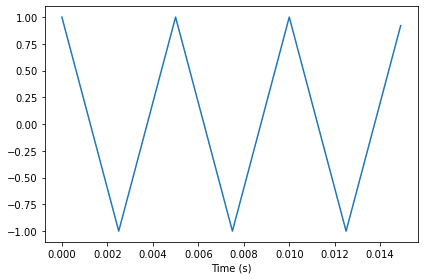
\includegraphics[width=0.75\textwidth]{tri_segment.png}
		\caption{Треугольный сигнал}
		\label{fig:tri_segment}
	\end{figure}
	\begin{lstlisting}[language=Python,caption=Построение спектра сигнала]
		wave = signal.make_wave(duration = 0.5, framerate = 10000)
		wave.apodize()
		spectrum = wave.make_spectrum()
		spectrum.plot()
	\end{lstlisting}
	\begin{figure}[H]
		\centering
		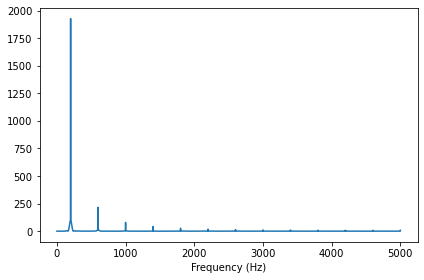
\includegraphics[width=0.75\textwidth]{tri_spectrum.png}
		\caption{Спектр треугольного сигнала}
		\label{fig:tri_spectrum}
	\end{figure}
	Амплитуда спадает пропорционально квадрату частоты.

	\begin{lstlisting}[language=Python,caption=Построение прямоугольного сигнала]
		from thinkdsp import SquareSignal

		signal = SquareSignal(200)
		duration = signal.period * 3
		segment = signal.make_wave(duration, framerate = 10000)
		segment.plot()
	\end{lstlisting}
	\begin{figure}[H]
		\centering
		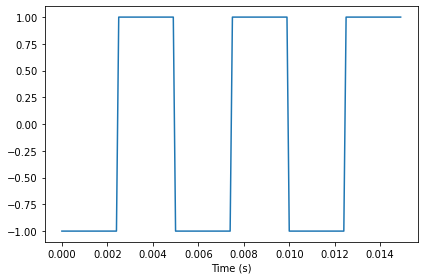
\includegraphics[width=0.75\textwidth]{sq_segment.png}
		\caption{Прямоугольный сигнал}
		\label{fig:sq_segment}
	\end{figure}
	\begin{figure}[H]
		\centering
		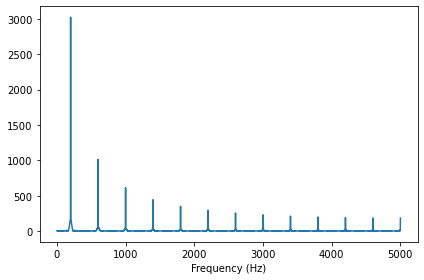
\includegraphics[width=0.75\textwidth]{sq_spectrum.png}
		\caption{Спектр прямоугольного сигнала}
		\label{fig:sq_spectrum}
	\end{figure}
	Амплитуда спадает пропорционально частоте (линейная зависимость).

	\chapter{Биения сигналов}
	Изучаем биения сигналов.
	\begin{lstlisting}[language=Python,caption=Построение косинусоиды с высокой частотой]
		from thinkdsp import CosSignal

		signal = CosSignal(5000)
		duration = signal.period * 5
		segment = signal.make_wave(duration, framerate = 10000)
		segment.plot()
	\end{lstlisting}
	\begin{figure}[H]
		\centering
		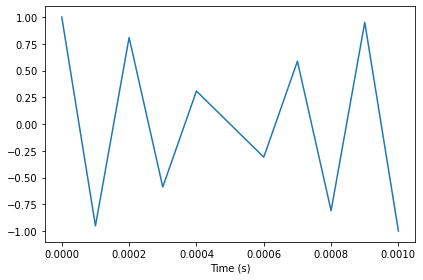
\includegraphics[width=0.75\textwidth]{aliasing1.png}
		\caption{Полученный сегмент сигнала}
		\label{fig:aliasing1}
	\end{figure}
	Если сигнал 5000 Гц и 10000 выборок в секунду, то количества выборок становится недостаточно, и теряется информация о сигнале. Это приводит к тому, что выборки из сигнала с высокой частотой кажутся выборками из сигнала с низкой частотой.

	\chapter{Функция для быстрого преобразования Фурье}
	Изучим работу функций \texttt{fft} и \texttt{rfft}.
	\begin{lstlisting}[language=Python,caption=Функция для быстрого преобразования Фурье]
		import numpy as np

		hs = np.fft.rfft(wave.ys)
		n = len(wave.ys)
		d = 1 / wave.framerate
		fs = np.fft.rfftfreq(n, d)
		magnitude = np.absolute(hs)
		plt.plot(fs, magnitude)
	\end{lstlisting}
	\begin{figure}[H]
		\centering
		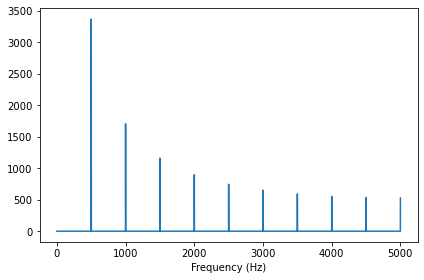
\includegraphics[width=0.75\textwidth]{spectrum1.png}
		\caption{Спектр сигнала после быстрого преобразования Фурье}
		\label{fig:spectrum1}
	\end{figure}

	\chapter{Изменение фазы сигнала}
	Перемешали фазы сигнала и изменили углы спектра.
	\begin{lstlisting}[language=Python,caption=Изменение сигнала]
		import random
		random.shuffle(angle)
		i = complex(0, 1)
		spectrum = wave.make_spectrum()
		spectrum.hs = magnitude * np.exp(i * angle)
		wave2 = spectrum.make_wave()
		wave2.normalize()
		segment = wave2.segment(duration = 0.005)
		segment.plot()
	\end{lstlisting}
	\begin{figure}[H]
		\centering
		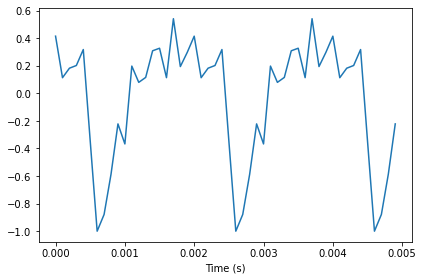
\includegraphics[width=0.75\textwidth]{segment1.png}
		\caption{Результат изменения исходного сигнала}
		\label{fig:segment1}
	\end{figure}

	\chapter{Упражнения}
	\section{Задание 2}
	Создаем и изучаем пилообразный сигнал
	\begin{lstlisting}[language=Python,caption=Получение пилообразного сигнала]
		from thinkdsp import Sinusoid
		from thinkdsp import normalize, unbias
		import numpy as np

		class SawtoothSignal(Sinusoid):
    
    			def evaluate(self, ts):
        			cycles = self.freq * ts + self.offset / np.pi / 2
       			frac, _ = np.modf(cycles)
        			ys = normalize(unbias(frac), self.amp)
        			return ys
		
		sawtooth = SawtoothSignal().make_wave(duration = 0.5, framerate = 20000)
		sawtooth.make_spectrum().plot()
	\end{lstlisting}
	\begin{figure}[H]
		\centering
		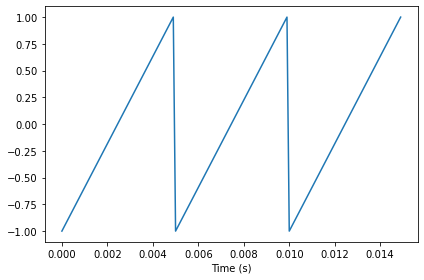
\includegraphics[width=0.75\textwidth]{pil_segment.png}
		\caption{Пилообразный сигнал}
		\label{fig:pil_segment}
	\end{figure}
	\begin{figure}[H]
		\centering
		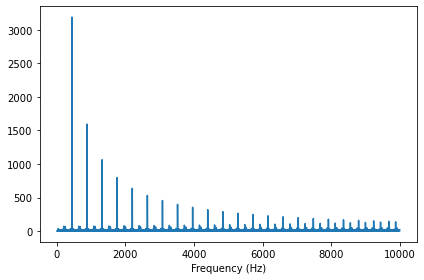
\includegraphics[width=0.75\textwidth]{pil_spectrum.png}
		\caption{Спектр пилообразного сигнала}
		\label{fig:pil_spectrum}
	\end{figure}
	\begin{figure}[H]
		\centering
		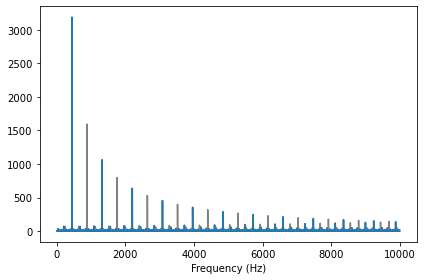
\includegraphics[width=0.75\textwidth]{sr1.png}
		\caption{Сравнение спектра пилообразного сигнала со спектром прямоугольного сигнала}
		\label{fig:sr1}
	\end{figure}
	\begin{figure}[H]
		\centering
		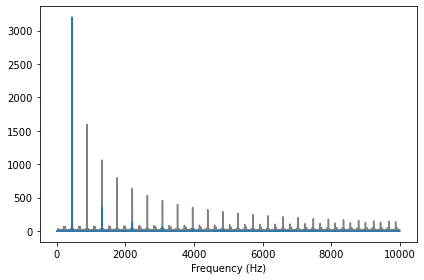
\includegraphics[width=0.75\textwidth]{sr2.png}
		\caption{Сравнение спектра пилообразного сигнала со спектром треугольного сигнала}
		\label{fig:sr2}
	\end{figure}
	Гармоники треугольного сигнала падают пропорционально $\frac{1}{f^2}$, в то время как гармоники пилообразного сигнала падают пропорционально $\frac{1}{f}$, но по сравнению с прямоугольным сигналом пилообразный сигнал включает в себя как четные, так и нечетные гармоники.

	\section{Задание 3}
	Создаём прямоугольный сигнал и проверяем его на биения.
	\begin{lstlisting}[language=Python,caption=Построение прямоугольного сигнала]
		square = SquareSignal(1100).make_wave(duration = 0.5, framerate = 10000)
		square.make_spectrum().plot()
	\end{lstlisting}
	\begin{figure}[H]
		\centering
		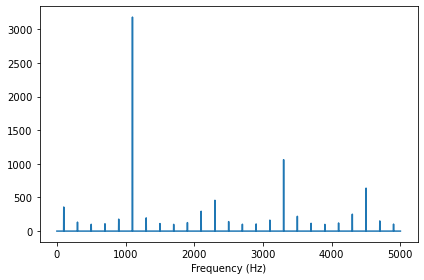
\includegraphics[width=0.75\textwidth]{spectrum2.png}
		\caption{Спектр прямоугольного сигнала с биениями}
		\label{fig:spectrum2}
	\end{figure}
	Создав сигнал с большей частотой дискретизации и сравнив эти два сигнала, мы услышим разницу между ними. Значит, биения влияют на качество сигнала.
	
	\section{Задание 4}
	Эксперимент с изменением амплитуды компоненты с частотой 0.
	 \begin{lstlisting}[language=Python,caption=Создаем треугольный сигнал]
		triangle = TriangleSignal(440).make_wave(duration=0.01)
		triangle.plot()
	\end{lstlisting}
	\begin{figure}[H]
		\centering
		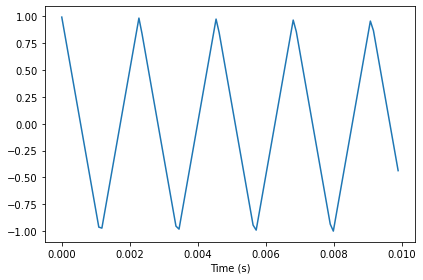
\includegraphics[width=0.75\textwidth]{segment2.png}
		\caption{Сигнал до изменений}
		\label{fig:segment2}
	\end{figure}
		Амплитуда и фаза нулевого компонента равнялись 0 (с небольшой погрешностью)
	\begin{lstlisting}[language=Python,caption=Изменяем амплитуду]
		spectrum = triangle.make_spectrum()
		spectrum.hs[0] = 100
		triangle.plot(color = 'gray')
		spectrum.make_wave().plot()
	\end{lstlisting}
	\begin{figure}[H]
		\centering
		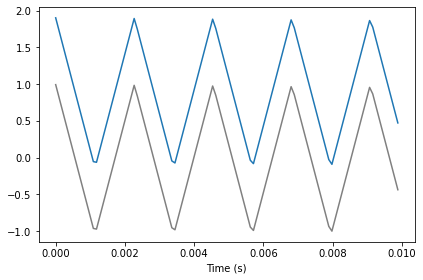
\includegraphics[width=0.75\textwidth]{sr3.png}
		\caption{Сравнение полученных сигналов}
		\label{fig:sr3}
	\end{figure}
	В результате сигнал оказался смещен вверх по амплитуде.
	
	\section{Задание 5}
	Функция для деления амплитуды сигнала на его частоту.
	 \begin{lstlisting}[language=Python,caption=Сама функция]
		def filter_spectrum(spectrum):
   			spectrum.hs[0] = 0
   			spectrum.hs[1:] /= spectrum.fs[1:]

		wave = TriangleSignal(freq=440).make_wave(duration=0.5)
		spectrum = wave.make_spectrum()
		spectrum.plot(high = 10000, color = 'gray')
		filter_spectrum(spectrum)
		spectrum.scale(440)
		spectrum.plot(high = 10000)
	\end{lstlisting}
	\begin{figure}[H]
		\centering
		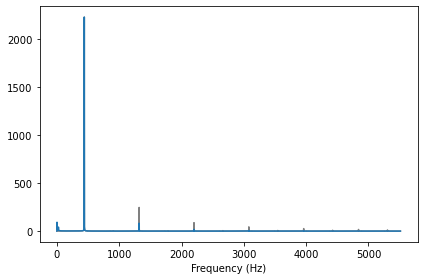
\includegraphics[width=0.75\textwidth]{test1.png}
		\caption{Применение этой функции для треугольного сигнала}
		\label{fig:test1}
	\end{figure}
	\begin{lstlisting}[language=Python,caption=Теперь возьмём прямоугольный сигнал]
		wave = SquareSignal(freq = 440).make_wave(duration=0.5)
		wave.make_audio()
		spectrum = wave.make_spectrum()
		spectrum.plot(high = 10000, color = 'gray')
		filter_spectrum(spectrum1)
		spectrum.scale(440)
		spectrum.plot(high = 10000)
	\end{lstlisting}
	\begin{figure}[H]
		\centering
		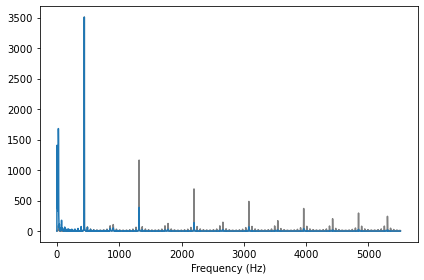
\includegraphics[width=0.75\textwidth]{test2.png}
		\caption{Применение этой функции для прямоугольного сигнала}
		\label{fig:test2}
	\end{figure}
	Полученные сигналы стали звучать как синосоидальный сигнал.

	\section{Задание 6}
	Ищем сигнал с четными и нечетными гармониками, спадающих пропорционально  $\frac{1}{f^2}$.
	 \begin{lstlisting}[language=Python,caption=Взяли пилообразный сигнал и уменьшили его амплитуду]
		signal = SawtoothSignal(freq = 1000)
		wave = signal.make_wave(duration=0.5, framerate=20000)
		spectrum = wave.make_spectrum()
		spectrum.plot(color = 'gray')
		filter_spectrum(spectrum)
		spectrum.scale(1000)
		spectrum.plot()
		wave = spectrum.make_wave()
		wave.segment(duration = 0.01).plot()
	\end{lstlisting}
	\begin{figure}[H]
		\centering
		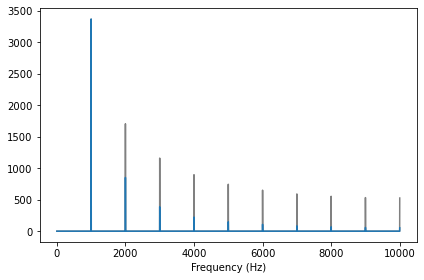
\includegraphics[width=0.75\textwidth]{result1.png}
		\caption{Полученный спектр}
		\label{fig:result1}
	\end{figure}
	\begin{figure}[H]
		\centering
		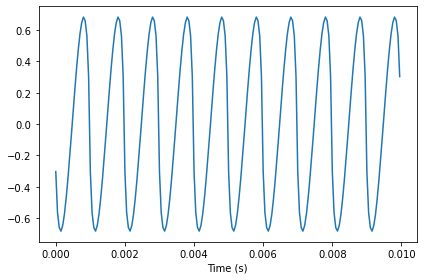
\includegraphics[width=0.75\textwidth]{result2.png}
		\caption{Полученный сигнал}
		\label{fig:result2}
	\end{figure}
	Получился сигнал странной формы, но с заданными свойствами. 
	\begin{lstlisting}[language=Python,caption=Второй способ]
		from thinkdsp import CosSignal

		freqs = np.arange(500, 9500, 500)
		amps = 1 / freqs ** 2
		signal = sum(CosSignal(freq, amp) for freq, amp in zip(freqs, amps))
		spectrum = wave.make_spectrum()
		spectrum.plot()
		wave = signal.make_wave(duration=0.5, framerate=20000)
		wave.segment(duration = 0.01).plot()
	\end{lstlisting}
	\begin{figure}[H]
		\centering
		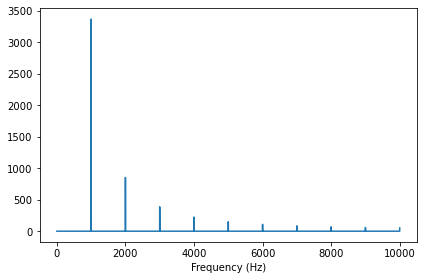
\includegraphics[width=0.75\textwidth]{test3.png}
		\caption{Нужный спектр}
		\label{fig:test3}
	\end{figure}
	\begin{figure}[H]
		\centering
		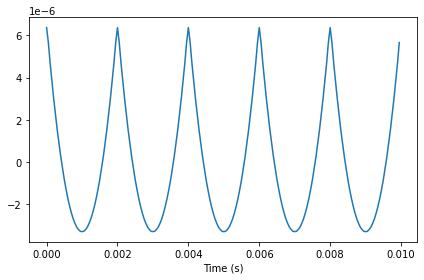
\includegraphics[width=0.75\textwidth]{test4.png}
		\caption{Странный сигнал}
		\label{fig:test4}
	\end{figure}
	В результате получился \texttt{ParabolicSignal} с заданными свойствами.
	
	\chapter{Вывод}
	В данной работе мы познакомились с треугольным, прямоугольным и пилообразным сигналами и посмотрели их спектры. Также мы узнали, что биения сигнала влияют на его качество.
\end{document}